\documentclass[aspectratio=169, lualatex]{beamer}
\makeatletter\def\input@path{{theme/}}\makeatother\usetheme{cipher}

\title{Applied Cryptography - 1.3: Provable Security \& Computational Cryptography}
\author{Nadim Kobeissi}
\subject{Foundations of provable security and computational cryptography in modern cryptographic systems.}
\keywords{provable security, computational cryptography, one-time pad, indistinguishability, libraries, subroutines, symmetric-key encryption, negligible functions, polynomial time, birthday paradox, bad event technique}
\institute{American University of Beirut}
\instituteimage{images/aub-white.png}
\date{\today}
\coversubtitle{CMPS 297AD/396AI\\Fall 2025}
\coverpartname{Part 1: Provable Security}
\covertopicname{1.3: Provable Security \\ \& Computational Cryptography}
\coverwebsite{https://appliedcryptography.page}

\begin{document}
\begin{frame}[plain]
	\titlepage
\end{frame}

\section{Provable Security}

\begin{frame}{Last time, we defined subroutines}
	\begin{center}
		\begin{tikzpicture}[
				box/.style={rectangle, draw, minimum height=2.5cm, align=left, fill=white},
				dashed box/.style={rectangle, draw, dashed, minimum width=2.5cm, minimum height=2.5cm, align=center, fill=white},
				>=Stealth,
			]
			\node[dashed box] (adversary) {$adversary$};
			\node[box, right=2cm of adversary](attack){
				$\underline{\func{attack}{M}}$: \hfill \quad \quad \textcolor{gray}{\scriptsize \textit{// adversary chooses $M$}} \\
				\quad $K \twoheadleftarrow \bits^{n}$ \hfill \quad \quad \textcolor{gray}{\scriptsize \textit{// victim samples $K$}} \\
				\quad $C \coloneq \textsf{Enc}(K, M)$ \hfill \quad \quad \textcolor{gray}{\scriptsize \textit{// victim encrypts}} \\
				\quad return $C$ \hfill \quad \quad \textcolor{gray}{\scriptsize \textit{// adversary sees $C$}}
			};
			\draw[->] (adversary) -- node[above] {$M$} (attack);
			\draw[<-] ([yshift=-0.5cm]adversary.east) -- node[below] {$C$} ([yshift=-0.5cm]attack.west);
		\end{tikzpicture}
	\end{center}
\end{frame}

\begin{frame}{Subroutines}
	\begin{columns}[c]
		\begin{column}{0.5\textwidth}
			\begin{itemize}
				\item ``Victim'' chooses their key.
				\item Adversary chooses the message and receives the ciphertext.
				\item We say that \textbf{the adversary has access to an encryption oracle}.
			\end{itemize}
		\end{column}
		\begin{column}{0.5\textwidth}
			\imagewithcaption{attacker-interface.pdf}{Source: The Joy of Cryptography}
		\end{column}
	\end{columns}
\end{frame}

\begin{frame}{Attack scenarios as libraries}
	\begin{columns}[c]
		\begin{column}{0.65\textwidth}
			\begin{itemize}
				\item This is a \textbf{library} with two \textbf{subroutines} and a \textbf{global variable} $D$.
				\item Victim holds a 6-sided die.
				\item The first line of the library represents an initialization step.
				\item Attacker can call the subroutines at any time, and:
				      \begin{enumerate}
					      \item Make a guess about the current value of the die and learn whether the guess was correct.
					      \item Instruct the victim to (privately) re-roll the die.
				      \end{enumerate}
			\end{itemize}
		\end{column}
		\begin{column}{0.35\textwidth}
			\vspace{-1cm}
			\begin{center}
				\sslibrary{}{dice-guess}{
					$D \twoheadleftarrow \{1, 2, 3, 4, 5, 6\}$ \\[1em]
					\sslibrarysubroutine{guess}{G}{
						return $D == G$
					}{1} \\[1em]
					\sslibrarysubroutine{reroll}{G}{
						$D \twoheadleftarrow \{1, 2, 3, 4, 5, 6\}$
					}{1}
				}{1}
			\end{center}
		\end{column}
	\end{columns}
\end{frame}

\begin{frame}{One-time pad}{From the adversary's perspective\ldots}
	\begin{columns}[c]
		\begin{column}{0.35\textwidth}
			\sssubroutine{Attack}{M}{
				$K \twoheadleftarrow \bits^{n}$ \\
				$C \coloneq K \oplus M$ \\
				return $C$
			}{1.5}
		\end{column}
		\begin{column}{0.3\textwidth}
			\begin{center}
				{\huge{$\approxeq$}} \\[1em]
				{\scriptsize\textit{(indistinguishable \\ from)}}
			\end{center}
		\end{column}
		\begin{column}{0.35\textwidth}
			\sssubroutine{Junk}{M}{
				$C \twoheadleftarrow \bits^{n}$ \\
				return $C$
			}{2}
		\end{column}
	\end{columns}
\end{frame}

\begin{frame}
	\begin{center}
		\huge \textit{``Real or random?''}
	\end{center}
\end{frame}

\begin{frame}{Programs and libraries}
	\begin{columns}[c]
		\begin{column}{0.5\textwidth}
			\begin{itemize}
				\item \prog{} is a \textbf{program} that calls \textbf{library} \lib{}{dice-guess}.
				\item Programs can only see the output of function calls to libraries.
				      \begin{itemize}
					      \item Programs can't read the values of library variables,
					      \item Programs can't measure how long it took to run a subroutine,
					      \item Etc.
				      \end{itemize}
			\end{itemize}
		\end{column}
		\begin{column}{0.5\textwidth}
			\sslinked{
				\ssprogram{}{
					if \func{guess}{6}:\\
					\quad return true\\
					\func{reroll}{}\\
					return \func{guess}{6}
				}{0.95}
			}{\link}{
				\sslibrary{}{dice-guess}{
					$D \twoheadleftarrow \{1, 2, 3, 4, 5, 6\}$ \\[1em]
					\sslibrarysubroutine{guess}{G}{
						return $D == G$
					}{1} \\[1em]
					\sslibrarysubroutine{reroll}{G}{
						$D \twoheadleftarrow \{1, 2, 3, 4, 5, 6\}$
					}{1}
				}{0.95}
			}
		\end{column}
	\end{columns}
\end{frame}

\begin{frame}{When are libraries interchangeable?}
	\begin{columns}[c]
		\begin{column}{0.55\textwidth}
			\begin{itemize}
				\item Libraries are \textbf{interchangeable} when they:
				      \begin{itemize}
					      \item Have the same interface,
					      \item \prob{\prog{}\link\lib{}{1} \Rightarrow \texttt{true}} $=$ \prob{\prog{}\link\lib{}{2} \Rightarrow \texttt{true}}
				      \end{itemize}
				\item i.e. when their usage and output is indistinguishable from the adversary's perspective when they are paired with \prog{}.
				\item A lot of the time, \prog{}'s mission is to try to \textit{distinguish} between \lib{}{1} and \lib{}{2}.
			\end{itemize}
		\end{column}
		\begin{column}{0.45\textwidth}
			\begin{flushright}
				\sslinked{
					\sslibrary{}{otp-real}{
						\sslibrarysubroutine{otp.enc}{M}{
							$K \twoheadleftarrow \bits^{n}$ \\
							$C \coloneq K \oplus M$ \\
							return $C$
						}{1}
					}{1}
				}{\interchangeable{}}{
					\sslibrary{}{otp-rand}{
						\sslibrarysubroutine{otp.enc}{M}{
							$R \twoheadleftarrow \bits^{n}$ \\
							return $R$
						}{1}
					}{1}
				}
			\end{flushright}
		\end{column}
	\end{columns}
\end{frame}

\begin{frame}{When are libraries interchangeable?}
	\begin{columns}[c]
		\begin{column}{0.5\textwidth}
			\begin{itemize}[<+->]
				\item Are these libraries interchangeable?
				\item \textbf{Yes!} Their only difference happens in \textit{unreachable lines of code}.
			\end{itemize}
		\end{column}
		\begin{column}{0.05\textwidth}
		\end{column}
		\begin{column}{0.45\textwidth}
			\sslinked{
				\sslibrary{}{a}{
					\sslibrarysubroutine{foo}{M}{
						$X \twoheadleftarrow \{1, \ldots, n\}$ \\
						if $X < 0$: \\
						\quad return $\bit{0}^n$
					}{1}
				}{1}
			}{\interchangeable{?}}{
				\sslibrary{}{b}{
					\sslibrarysubroutine{foo}{M}{
						$X \twoheadleftarrow \{1, \ldots, n\}$ \\
						if $X < 0$: \\
						\quad return $\bit{0}^1$
					}{1}
				}{1}
			}
		\end{column}
	\end{columns}
\end{frame}

\begin{frame}{When are libraries interchangeable?}
	\begin{columns}[c]
		\begin{column}{0.5\textwidth}
			\begin{itemize}[<+->]
				\item Are these libraries interchangeable?
				\item \textbf{Yes!} Their only difference is the value they assign to a \textit{variable that is never actually used}.
			\end{itemize}
		\end{column}
		\begin{column}{0.05\textwidth}
		\end{column}
		\begin{column}{0.45\textwidth}
			\sslinked{
				\sslibrary{}{a}{
					\sslibrarysubroutine{foo}{A, B}{
						$Y \twoheadleftarrow \bits^n$\\
						$C \coloneq \func{bar}{A}$\\
						return $Y$
					}{1}\\[1em]
					\sslibrarysubroutine{bar}{M}{
						$X \twoheadleftarrow \bits^n$\\
						return $X$
					}{1}
				}{1}
			}{\interchangeable{?}}{
				\sslibrary{}{b}{
					\sslibrarysubroutine{foo}{A, B}{
						$Y \twoheadleftarrow \bits^n$\\
						$C \coloneq \func{bar}{B}$\\
						return $Y$
					}{1}\\[1em]
					\sslibrarysubroutine{bar}{M}{
						$X \twoheadleftarrow \bits^n$\\
						return $X$
					}{1}
				}{1}
			}
		\end{column}
	\end{columns}
\end{frame}

\begin{frame}{When are libraries interchangeable?}
	\begin{columns}[c]
		\begin{column}{0.5\textwidth}
			\begin{itemize}[<+->]
				\item Are these libraries interchangeable?
				\item $\|$ denotes string concatenation.
				      \begin{itemize}
					      \item $\texttt{Po} \| \texttt{tato} = \texttt{Potato}$
				      \end{itemize}
				\item \textbf{Yes!} Outputting the concatentaion two randomly sampled uniform strings of lengths $n$ and $m$ is the same as outputting a single random string of length $n + m$.
			\end{itemize}
		\end{column}
		\begin{column}{0.05\textwidth}
		\end{column}
		\begin{column}{0.45\textwidth}
			\sslinked{
				\sslibrary{}{a}{
					\sslibrarysubroutine{sample}{}{
						$X \twoheadleftarrow \bits^n$\\
						$Y \twoheadleftarrow \bits^m$\\
						return $X \| Y$
					}{1}
				}{1}
			}{\interchangeable{?}}{
				\sslibrary{}{b}{
					\sslibrarysubroutine{sample}{}{
						$R \twoheadleftarrow \bits^{n+m}$\\
						return $R$
					}{1}
				}{1}
			}
		\end{column}
	\end{columns}
\end{frame}

\begin{frame}{When are libraries interchangeable?}
	\begin{columns}[c]
		\begin{column}{0.5\textwidth}
			\begin{itemize}[<+->]
				\item Are these libraries interchangeable?
				\item \textbf{No!} The first library uses the same $K$ for all subsequent encryptions, which breaks OTP security.
				      \begin{itemize}
					      \item Recall that OTP requires keys to be only used once (hence the name).
				      \end{itemize}
			\end{itemize}
		\end{column}
		\begin{column}{0.05\textwidth}
		\end{column}
		\begin{column}{0.45\textwidth}
			\sslinked{
				\sslibrary{}{a}{
					$K \twoheadleftarrow \bits^n$\\[1em]
					\sslibrarysubroutine{otp.enc}{M}{
						$C \coloneq K \oplus M$ \\
						return $C$
					}{1}
				}{1}
			}{\interchangeable{?}}{
				\sslibrary{}{b}{
					\sslibrarysubroutine{otp.enc}{M}{
						$C \twoheadleftarrow \bits^n$\\
						return $C$
					}{1}
				}{1}
			}
		\end{column}
	\end{columns}
\end{frame}

\begin{frame}{How do we show the distinguisher?}
	\begin{columns}[c]
		\begin{column}{0.4\textwidth}
			\begin{itemize}[<+->]
				\item What happens if we call \prog{}\link\lib{}{a} multiple times?
				      \begin{itemize}
					      \item We'll get the same output $\equiv K$ each time!
				      \end{itemize}
				\item \prob{\prog{}\link\lib{}{a} \Rightarrow \texttt{true}} $= 1$,
			\end{itemize}
		\end{column}
		\begin{column}{0.6\textwidth}
			\begin{flushright}
				\sslinked{
					\ssprogram{}{
						$C_1 \coloneq \func{otp.enc}{\bit{0}^n}$\\
						$C_2 \coloneq \func{otp.enc}{\bit{0}^n}$\\
						return $C_1 == C_2$
					}{1}
				}{\link}{
					\sslibrary{}{a}{
						$K \twoheadleftarrow \bits^n$\\[1em]
						\sslibrarysubroutine{otp.enc}{M}{
							$C \coloneq K \oplus M$ \\
							return $C$
						}{1}
					}{1}
				}
			\end{flushright}
		\end{column}
	\end{columns}
\end{frame}

\begin{frame}{How do we show the distinguisher?}
	\begin{columns}[c]
		\begin{column}{0.4\textwidth}
			\begin{itemize}
				\item What happens if we call \prog{}\link\lib{}{a} multiple times?
				      \begin{itemize}
					      \item We'll get the same output $\equiv K$ each time!
				      \end{itemize}
				\item \prob{\prog{}\link\lib{}{a} \Rightarrow \texttt{true}} $= 1$,
				\item \prob{\prog{}\link\lib{}{b} \Rightarrow \texttt{true}} $= \frac{1}{2^n}$.
			\end{itemize}
		\end{column}
		\begin{column}{0.6\textwidth}
			\begin{flushright}
				\sslinked{
					\ssprogram{}{
						$C_1 \coloneq \func{otp.enc}{\bit{0}^n}$\\
						$C_2 \coloneq \func{otp.enc}{\bit{0}^n}$\\
						return $C_1 == C_2$
					}{1}
				}{\link}{
					\sslibrary{}{b}{
						\sslibrarysubroutine{otp.enc}{M}{
							$C \twoheadleftarrow \bits^n$\\
							return $C$
						}{1}
					}{1}
				}
			\end{flushright}
		\end{column}
	\end{columns}
\end{frame}

\begin{frame}{OTP: why key re-use is bad}
	\begin{columns}[c]
		\begin{column}{0.5\textwidth}
			\begin{align*}
				C_i \oplus C_j & = (K \oplus M_i) \oplus (K \oplus M_j) \\
				               & = K \oplus K \oplus M_i \oplus M_j     \\
				               & = \bit{0}^n \oplus M_i \oplus M_j      \\
				               & = M_i \oplus M_j
			\end{align*}
			\begin{itemize}
				\item \prob{\prog{}\link\lib{}{a} \Rightarrow \texttt{true}} $= 1$\footnote{Interactive demo: \url{https://www.douglas.stebila.ca/teaching/visual-one-time-pad/}}
			\end{itemize}
		\end{column}
		\begin{column}{0.5\textwidth}
			\begin{flushright}
				\sslinked{
					\ssprogram{}{
						$M_1 \twoheadleftarrow \bits^n$\\
						$M_2 \twoheadleftarrow \bits^n$\\
						$C_1 \coloneq \func{otp.enc}{M_1}$\\
						$C_2 \coloneq \func{otp.enc}{M_2}$\\
						return $C_1 \oplus C_2 == M_1 \oplus M_2$
					}{0.85}
				}{\link}{
					\sslibrary{}{a}{
						$K \twoheadleftarrow \bits^n$\\[1em]
						\sslibrarysubroutine{otp.enc}{M}{
							$C \coloneq K \oplus M$ \\
							return $C$
						}{1}
					}{0.85}
				}
			\end{flushright}
		\end{column}
	\end{columns}
\end{frame}

\begin{frame}{Proving two libraries are interchangeable}
	\begin{columns}[c]
		\begin{column}{0.5\textwidth}
			\begin{itemize}[<+->]
				\item Are these libraries interchangeable?
				\item Let's find out!
				\item \textbf{Goal:} transform \lib{}{xor-samp-1} to \lib{}{xor-samp-2}, proving that each transformation step does not cause any change whatsoever to the library's functionality.
			\end{itemize}
		\end{column}
		\begin{column}{0.5\textwidth}
			\begin{flushright}
				\sslinked{
					\sslibrary{}{xor-samp-1}{
						\sslibrarysubroutine{sample}{M}{
							$X \twoheadleftarrow \bits^n$ \\
							$Y \coloneq X \oplus M$ \\
							return $(X, Y)$
						}{1}
					}{1}
				}{\interchangeable{?}}{
					\sslibrary{}{xor-samp-2}{
						\sslibrarysubroutine{sample}{M}{
							$Y \twoheadleftarrow \bits^n$ \\
							$X \coloneq Y \oplus M$ \\
							return $(X, Y)$
						}{1}
					}{1}
				}
			\end{flushright}
		\end{column}
	\end{columns}
\end{frame}

\begin{frame}{Proving two libraries are interchangeable}{Step 1}
	\begin{columns}[c]
		\begin{column}{0.5\textwidth}
			\begin{itemize}
				\item We start at \lib{}{xor-samp-1}.
			\end{itemize}
		\end{column}
		\begin{column}{0.5\textwidth}
			\begin{center}
				\sslibrary{}{xor-samp-1}{
					\sslibrarysubroutine{sample}{M}{
						$X \twoheadleftarrow \bits^n$ \\
						$Y \coloneq X \oplus M$ \\
						return $(X, Y)$
					}{1}
				}{1}
			\end{center}
		\end{column}
	\end{columns}
\end{frame}

\begin{frame}{Proving two libraries are interchangeable}{Step 2}
	\begin{columns}[c]
		\begin{column}{0.5\textwidth}
			\begin{itemize}
				\item Let's add a new variable $X'$.
				\item Note that $X = X'$:
				      \begin{itemize}
					      \item $X' = Y \oplus M = (X \oplus M) \oplus M = X$.
				      \end{itemize}
			\end{itemize}
		\end{column}
		\begin{column}{0.5\textwidth}
			\begin{center}
				\sslibrary{}{hyb-1}{
					\sslibrarysubroutine{sample}{M}{
						$X \twoheadleftarrow \bits^n$ \\
						$Y \coloneq X \oplus M$ \\
						\hl{$X' \coloneq Y \oplus M$} \\
						return $(X, Y)$
					}{1}
				}{1}
			\end{center}
		\end{column}
	\end{columns}
\end{frame}

\begin{frame}{Proving two libraries are interchangeable}{Step 3}
	\begin{columns}[c]
		\begin{column}{0.5\textwidth}
			\begin{itemize}
				\item So, we can return $(X', Y)$ without any change on the library's effect.
				      \begin{itemize}
					      \item $X' = Y \oplus M = (X \oplus M) \oplus M = X$.
				      \end{itemize}
			\end{itemize}
		\end{column}
		\begin{column}{0.5\textwidth}
			\begin{center}
				\sslibrary{}{hyb-2}{
					\sslibrarysubroutine{sample}{M}{
						$X \twoheadleftarrow \bits^n$ \\
						$Y \coloneq X \oplus M$ \\
						$X' \coloneq Y \oplus M$ \\
						\hl{return $(X', Y)$}
					}{1}
				}{1}
			\end{center}
		\end{column}
	\end{columns}
\end{frame}

\begin{frame}{Proving two libraries are interchangeable}{Step 4}
	\begin{columns}[c]
		\begin{column}{0.5\textwidth}
			\begin{itemize}
				\item The first two lines of \func{sample}{M} are the same as \func{otp.enc}{M}, so we link it and use it instead.
			\end{itemize}
		\end{column}
		\begin{column}{0.5\textwidth}
			\begin{center}
				\sslinked{
					\sslibrary{}{hyb-3-4}{
						\sslibrarysubroutine{sample}{M}{
							\hl{$Y \coloneq \func{otp.enc}{M}$} \\
							$X' \coloneq Y \oplus M$ \\
							return $(X', Y)$
						}{1}
					}{1}
				}{\link}{
					\sslibrary{}{otp-real}{
						\sslibrarysubroutine{otp.enc}{M}{
							$K \twoheadleftarrow \bits^n$ \\
							$C \coloneq K \oplus M$ \\
							return $C$
						}{1}
					}{1}
				}
			\end{center}
		\end{column}
	\end{columns}
\end{frame}

\begin{frame}{Proving two libraries are interchangeable}{Step 5}
	\begin{columns}[c]
		\begin{column}{0.5\textwidth}
			\begin{itemize}
				\item The first two lines of \func{sample}{M} are the same as \func{otp.enc}{M}, so we link it and use it instead.
				\item Recall that \lib{}{otp-real} \interchangeable{} \lib{}{otp-rand}!
				\item So, we replace \lib{}{otp-real} with \lib{}{otp-rand}.
			\end{itemize}
		\end{column}
		\begin{column}{0.5\textwidth}
			\begin{center}
				\sslinked{
					\sslibrary{}{hyb-3-4}{
						\sslibrarysubroutine{sample}{M}{
							$Y \coloneq \func{otp.enc}{M}$ \\
							$X' \coloneq Y \oplus M$ \\
							return $(X', Y)$
						}{1}
					}{1}
				}{\link}{
					\sslibrary{}{otp-rand}{
						\sslibrarysubroutine{otp.enc}{M}{
							$R \twoheadleftarrow \bits^{n}$ \\
							return $R$
						}{1}
					}{1}
				}
			\end{center}
		\end{column}
	\end{columns}
\end{frame}

\begin{frame}{Proving two libraries are interchangeable}{Step 6}
	\begin{columns}[c]
		\begin{column}{0.5\textwidth}
			\begin{itemize}
				\item The first two lines of \func{sample}{M} are the same as \func{otp.enc}{M}, so we link it and use it instead.
				\item Recall that \lib{}{otp-real} \interchangeable{} \lib{}{otp-rand}!
				\item So, we replace \lib{}{otp-real} with \lib{}{otp-rand}.
				\item We inline \lib{}{otp-rand} back into our main library.
			\end{itemize}
		\end{column}
		\begin{column}{0.5\textwidth}
			\begin{center}
				\sslibrary{}{hyb-5}{
					\sslibrarysubroutine{sample}{M}{
						$Y \hl{\twoheadleftarrow \bits^n}$ \\
						$X' \coloneq Y \oplus M$ \\
						return $(X', Y)$
					}{1}
				}{1}
			\end{center}
		\end{column}
	\end{columns}
\end{frame}

\begin{frame}{Proving two libraries are interchangeable}{Step 7}
	\begin{columns}[c]
		\begin{column}{0.5\textwidth}
			\begin{itemize}
				\item The first two lines of \func{sample}{M} are the same as \func{otp.enc}{M}, so we link it and use it instead.
				\item Recall that \lib{}{otp-real} \interchangeable{} \lib{}{otp-rand}!
				\item So, we replace \lib{}{otp-real} with \lib{}{otp-rand}.
				\item We inline \lib{}{otp-rand} back into our main library.
				\item Finally, we rename $X'$ to $X$.
			\end{itemize}
		\end{column}
		\begin{column}{0.5\textwidth}
			\begin{center}
				\sslibrary{}{hyb-6}{
					\sslibrarysubroutine{sample}{M}{
						$Y \twoheadleftarrow \bits^n$ \\
						$\hl{X} \coloneq Y \oplus M$ \\
						return $(\hl{X}, Y)$
					}{1}
				}{1}
			\end{center}
		\end{column}
	\end{columns}
\end{frame}

\begin{frame}{Proving two libraries are interchangeable}{Result}
	\begin{columns}[c]
		\begin{column}{0.5\textwidth}
			\begin{itemize}
				\item Interchangeable!
				\item Note how we had to show equivalence \textbf{at each step}.
			\end{itemize}
		\end{column}
		\begin{column}{0.5\textwidth}
			\begin{center}
				\sslinked{
					\sslibrary{}{hyb-6}{
						\sslibrarysubroutine{sample}{M}{
							$Y \twoheadleftarrow \bits^n$ \\
							$X \coloneq Y \oplus M$ \\
							return $(X, Y)$
						}{1}
					}{1}
				}{\interchangeable{}}{
					\sslibrary{}{xor-samp-2}{
						\sslibrarysubroutine{sample}{M}{
							$Y \twoheadleftarrow \bits^n$ \\
							$X \coloneq Y \oplus M$ \\
							return $(X, Y)$
						}{1}
					}{1}
				}
			\end{center}
		\end{column}
	\end{columns}
\end{frame}

\begin{frame}{Cryptographic primitives}
	\begin{itemize}
		\item Specific algorithms like OTP are important in cryptography, but OTP is just one instance of an \textbf{encryption scheme}.
		\item In cryptography, useful abstractions like ``encryption scheme'' are called \textbf{primitives}.
		\item Three things are important when defining a cryptographic primitive:
		      \begin{enumerate}
			      \item \textbf{Syntax}: The basic raw interface - algorithms, inputs/outputs and their types.
			      \item \textbf{Correctness}: Basic functionality without adversaries - e.g., ``decryption should be the inverse of encryption''.
			      \item \textbf{Security}: Guarantees that hold in specific attack scenarios with adversaries.
		      \end{enumerate}
	\end{itemize}
\end{frame}

\begin{frame}{Cryptographic primitives}{$\Sigma$: a symmetric-key encryption scheme}
	\begin{itemize}
		\item \textbf{$\Sigma.\textsf{KeyGen}() = K$}
		      \begin{itemize}
			      \item Input: none
			      \item Output: key $K \in \Sigma.\mathcal{K}$ {\tiny(the ``key space'')}.
		      \end{itemize}
		\item \textbf{$\Sigma.\textsf{Enc}(K, M) = C$}
		      \begin{itemize}
			      \item Input: key $K \in \Sigma.\mathcal{K}$, plaintext $M \in \Sigma.\mathcal{M}$ {\tiny(the ``message space'')}.
			      \item Output: ciphertext $C \in \Sigma.\mathcal{C}$.
		      \end{itemize}
		\item \textbf{$\Sigma.\textsf{Dec}(K, C) = M$}
		      \begin{itemize}
			      \item Input: key $K \in \Sigma.\mathcal{K}$, ciphertext $C \in \Sigma.\mathcal{C}$ {\tiny(the ``ciphertext space'')}.
			      \item Output: plaintext $M \in \Sigma.\mathcal{M}$.
		      \end{itemize}
	\end{itemize}
\end{frame}

\begin{frame}{Correctness of a SKE}
	\begin{columns}[c]
		\begin{column}{0.5\textwidth}
			\definitionbox{Correctness for SKE}{
				An SKE scheme $\Sigma$ is correct if encryption and decryption are inverses, in the following sense:
				\begin{align*}
					\prob{\Sigma.\textsf{Dec}(K, \Sigma.\textsf{Enc}(K, M)) = M} = 1
				\end{align*}
				for all $M \in \Sigma.\mathcal{M}$ and $K \in \Sigma.\mathcal{K}$.
			}
		\end{column}
		\begin{column}{0.5\textwidth}
			\begin{itemize}
				\item The definition involves a probability because $\Sigma.\textsf{Enc}$ may be a randomized algorithm.
				\item This means that decryption should \textbf{always} recover the original message.
				\item Even if encryption adds randomness, decryption must be deterministic for each key-ciphertext pair.
			\end{itemize}
		\end{column}
	\end{columns}
\end{frame}

\begin{frame}{One-time secrecy of a SKE}
	\begin{columns}[c]
		\begin{column}{0.5\textwidth}
			\definitionbox{One-time Secrecy for SKE}{
				An SKE scheme $\Sigma$ has one-time secrecy if the following libraries are interchangeable:
				\vspace{0.5mm}
				\begin{center}
					\sslinked{
						\sslibrary{\Sigma}{ots-real}{
							\sslibrarysubroutine{ots.enc}{M}{
								$K \twoheadleftarrow \Sigma.\mathcal{K}$ \\
								$C \coloneq \Sigma.\textsf{Enc}(K, M)$ \\
								return $C$
							}{1}
						}{0.8}
					}{\interchangeable{}}{
						\sslibrary{\Sigma}{ots-rand}{
							\sslibrarysubroutine{ots.enc}{M}{
								$C \twoheadleftarrow \Sigma.\mathcal{C}$ \\
								return $C$
							}{1}
						}{0.8}
					}
				\end{center}
			}
		\end{column}
		\begin{column}{0.5\textwidth}
			An encryption scheme has one-time secrecy if its ciphertexts are uniformly distributed, when keys are sampled uniformly, kept secret, and used for only one encryption, and no matter how the plaintexts are chosen.
		\end{column}
	\end{columns}
\end{frame}

\begin{frame}{Reminder: AND $(\land)$}
	\begin{columns}[c]
		\begin{column}{0.7\textwidth}
			\begin{itemize}[<+->]
				\item Let's replace $\oplus$ with $\land$. What would happen?
				\item Output no longer uniform!
			\end{itemize}
			\begin{table}
				\centering
				\begin{tabular}{|c|c|c|}
					\hline
					\textbf{A} & \textbf{B} & \textbf{A $\land$ B} \\
					\hline
					\bit{0}    & \bit{0}    & \bit{0}              \\
					\hline
					\bit{0}    & \bit{1}    & \bit{0}              \\
					\hline
					\bit{1}    & \bit{0}    & \bit{0}              \\
					\hline
					\bit{1}    & \bit{1}    & \bit{1}              \\
					\hline
				\end{tabular}
				\caption{Truth table for AND operation}
			\end{table}
		\end{column}
		\begin{column}{0.3\textwidth}
			\sssubroutine{Attack}{M}{
				$K \twoheadleftarrow \bits^{n}$ \\
				$C \coloneq K \land M$ \\
				return $C$
			}{1.5}
		\end{column}
	\end{columns}
\end{frame}

\begin{frame}{Creating a distinguisher program}
	\begin{columns}[c]
		\begin{column}{0.5\textwidth}
			\begin{center}
				\sslinked{
					\sslibrary{}{ots-real}{
						\sslibrarysubroutine{ots.enc}{M}{
							$K \twoheadleftarrow \bits^n$ \\
							$C \coloneq K \land M$ \\
							return $C$
						}{1}
					}{1}
				}{\interchangeable{?}}{
					\sslibrary{}{ots-rand}{
						\sslibrarysubroutine{ots.enc}{M}{
							$C \twoheadleftarrow \bits^n$ \\
							return $C$
						}{1}
					}{1}
				}
			\end{center}
		\end{column}
		\begin{column}{0.5\textwidth}
			\begin{itemize}
				\item Can you write a distinguisher program showing that these libraries are \textbf{not} interchangeable?
				      \pause
				\item \ssprogram{}{
					      $M \coloneq \bit{0}^n$\\
					      $C \coloneq \func{ots.enc}{M}$\\
					      return $C == \bit{0}^n$
				      }{1}
				\item \prob{A\link\lib{}{ots-real} \Rightarrow \texttt{true}} $= 1$
				\item \prob{A\link\lib{}{ots-rand} \Rightarrow \texttt{true}} $= \frac{1}{2^n}$
			\end{itemize}
		\end{column}
	\end{columns}
\end{frame}

\section{Computational Cryptography}

\begin{frame}{Computational notions in cryptography}
	\begin{itemize}
		\item Security definitions in theoretical cryptography can be too strict:
		      \begin{itemize}
			      \item Even attacks requiring a trillion years of computation.
			      \item Even attacks with probability lower than winning the lottery 100 times.
		      \end{itemize}
		\item Modern provable security takes a more practical approach:
		      \begin{itemize}
			      \item We dismiss attacks with ``ridiculously'' high computational cost.
			      \item We dismiss attacks with ``ridiculously'' tiny success probability.
		      \end{itemize}
		\item Instead of ``no attack can succeed, not even in principle'',
		\item We prove: ``every attack has either ridiculously high cost or ridiculously small success probability''.
	\end{itemize}
\end{frame}

\begin{frame}{The concrete approach to provable security}
	\begin{itemize}
		\item In the concrete approach to provable security, we aim to be as quantitative as possible about security claims.
		\item We rarely say definitively that a cryptographic algorithm ``is secure'', as we did with OTP.
		\item Instead, we use statements like:
		      \begin{itemize}
			      \item \textit{``Any attack that expends at most $2^{80}$ effort can succeed with probability no better than $2^{-64}$.''}
		      \end{itemize}
		\item It is up to the user to judge whether this quantitative level of security is acceptable based on their use-case.
		\item This gives users a concrete basis for security decisions.
	\end{itemize}
\end{frame}

\subsection{Asymptotic approach to security}

\begin{frame}{Monetary cost of huge computations}
	\begin{itemize}
		\item One way to think about huge computations is their monetary cost.
		\item The table below shows roughly how much a computation involving $2^n$ CPU cycles would cost on the cheapest available Amazon EC2 cloud computing service:
	\end{itemize}
	\begin{table}
		\centering
		\begin{tabular}{cll}
			\textbf{Clock cycles} & \textbf{Approx cost (USD)} & \textbf{Point of reference}                      \\
			\hline
			$2^{50}$              & \$3.50                     & cup of coffee                                    \\
			$2^{55}$              & \$100                      & dinner at a high-end restaurant                  \\
			$2^{65}$              & \$130,000                  & apartment in Achrafieh                           \\
			$2^{75}$              & \$130 million              & budget of one of the Harry Potter movies         \\
			$2^{85}$              & \$140 billion              & GDP of Hungary                                   \\
			$2^{92}$              & \$20 trillion              & GDP of the United States                         \\
			$2^{99}$              & \$2 quadrillion            & all of human economic activity since 300,000 BCE \\
			$2^{128}$             & a lot!                     & a billion human civilizations' worth of effort   \\
		\end{tabular}
	\end{table}
\end{frame}

\begin{frame}{Exponential vs polynomial growth}{Quick side-note}
	\begin{columns}[c]
		\begin{column}{0.5\textwidth}
			\begin{itemize}
				\item Important insight: $2^{n+1} = 2 \times 2^n$
				      \begin{itemize}
					      \item $2^{51} = 2 \times 2^{50}$
					      \item $2^{128} = 2^{64} \times 2^{64}$
				      \end{itemize}
				\item Each additional bit doubles the computational cost!
				\item Compare growth rates:
				      \begin{itemize}
					      \item Linear: $f(n) = n$
					      \item Polynomial: $f(n) = n^2$
					      \item Exponential: $f(n) = 2^n$
				      \end{itemize}
			\end{itemize}
		\end{column}
		\begin{column}{0.5\textwidth}
			\begin{center}
				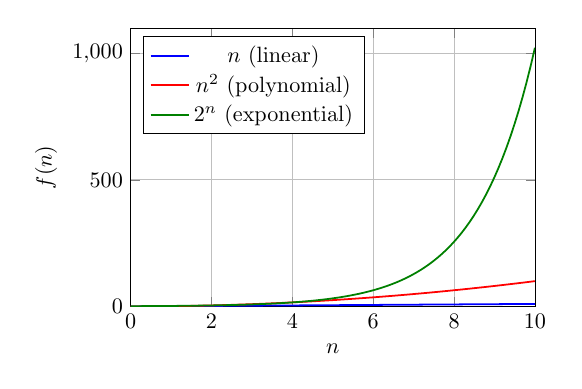
\begin{tikzpicture}[scale=0.8]
					\begin{axis}[
							xlabel={$n$},
							ylabel={$f(n)$},
							xmin=0, xmax=10,
							ymin=0, ymax=1100,
							legend pos=north west,
							grid=major,
							width=8cm,
							height=6cm,
						]
						\addplot[domain=0:10, samples=100, thick, blue] {x};
						\addlegendentry{$n$ (linear)}
						\addplot[domain=0:10, samples=100, thick, red] {x^2};
						\addlegendentry{$n^2$ (polynomial)}
						\addplot[domain=0:10, samples=100, thick, green!50!black] {2^x};
						\addlegendentry{$2^n$ (exponential)}
					\end{axis}
				\end{tikzpicture}
			\end{center}
			\textit{\small Note: Exponential growth quickly surpasses all polynomial functions!}
		\end{column}
	\end{columns}
\end{frame}

\begin{frame}{Understanding tiny probabilities}
	\begin{itemize}
		\item Let's put extremely small probabilities in perspective:
		      \begin{itemize}
			      \item In 2009, Patricia Demauro rolled dice 154 consecutive times without getting a 7 in craps.
			      \item Probability of this event: $(30/36)^{154} \approx 2^{-40.6}$
			      \item Often cited as one of the most improbable documented events in gambling history.
		      \end{itemize}
		\item Other extremely unlikely gambling events:
		      \begin{itemize}
			      \item In 1943, a roulette wheel reportedly landed on red 32 consecutive times.
			      \item Probability: $(18/38)^{31} \approx 2^{-33.4}$
			      \item Winning the American Powerball lottery: $2^{-28.1}$
			      \item Winning Powerball two consecutive weeks: $2^{-56.2}$
		      \end{itemize}
		\item These examples help us intuitively grasp what probabilities like $2^{-40}$ or $2^{-50}$ actually mean.
	\end{itemize}
\end{frame}

\begin{frame}{Why $2^{-x}$ for probabilities?}{Quick side-note}
	\begin{itemize}
		\item We've been using notation like $2^{-40}$, $2^{-64}$, $2^{-128}$ for probabilities. Why the negative exponent?
		\item Recall that $2^{-x} = \frac{1}{2^x}$
		      \begin{itemize}
			      \item $2^{-40} = \frac{1}{2^{40}} = \frac{1}{1,099,511,627,776}$
			      \item This is approximately 1 in a trillion
		      \end{itemize}
		\item Probabilities must be between 0 and 1:
		      \begin{itemize}
			      \item $2^{40}$ would be a huge number (over a trillion) - not a valid probability!
			      \item $2^{-40}$ is a tiny fraction - exactly what we want for unlikely events
		      \end{itemize}
	\end{itemize}
\end{frame}

\begin{frame}{Computational scale of Bitcoin mining}
	\begin{itemize}
		\item Let's consider cryptocurrencies based on proof-of-work, like Bitcoin.
		\item These systems incentivize users to perform truly obscene amounts of computation.
		\item In Bitcoin's proof-of-work mechanism:
		      \begin{itemize}
			      \item Users race to perform SHA-256 hash computations as fast as possible.
			      \item The collective Bitcoin network has performed approximately $2^{95}$ SHA-256 hashes in total.
			      \item In the last 12 months alone: approximately $2^{93.6}$ hashes.
			      \item Current market cap for Bitcoin: approximately 400 billion USD.
		      \end{itemize}
		\item This shows the enormous scale of computation that economic incentives can support.
	\end{itemize}
\end{frame}

\begin{frame}{The asymptotic approach to provable security}
	\begin{columns}
		\begin{column}{1\textwidth}
			\begin{itemize}
				\item The concrete approach gives practical guidance (e.g., key sizes) but requires managing tedious quantitative details.
				\item The asymptotic approach\footnote{Asymptotic means ``approaching a limit''. In computer science, we study how algorithms behave as input size approaches infinity, focusing on the general trend rather than exact values.}:
				      \begin{itemize}
					      \item Makes qualitative, all-or-nothing statements
					      \item Considers behavior as key size approaches infinity
					      \item Hides tedious quantitative details
				      \end{itemize}
				\item Similar to asymptotic analysis using big-O notation.
				\item Example: Instead of calculating that an operation takes exactly $16n^2 + 24n + 74$ steps, we can simply say it takes $\mathcal{O}(n^2)$ steps
			\end{itemize}
		\end{column}
	\end{columns}
\end{frame}

\begin{frame}{AES: An example of asymptotic security analysis}
	\begin{columns}[c]
		\begin{column}{0.5\textwidth}
			\begin{itemize}
				\item The Advanced Encryption Standard (AES) is a common symmetric-key encryption algorithm.
				\item It comes in different variants: AES-128, AES-192, AES-256.
				\item In asymptotic analysis, we'd say:
				      \begin{itemize}
					      \item AES is secure against all polynomial-time adversaries.
					      \item Any successful attack must take exponential time in the key length.
				      \end{itemize}
				\item This hides the concrete details about specific computational costs.
			\end{itemize}
		\end{column}
		\begin{column}{0.5\textwidth}
			\begin{itemize}
				\item Concrete security for AES-128:
				      \begin{itemize}
					      \item Best known attack: $\approx 2^{126.1}$ operations
				      \end{itemize}
				\item For AES-256:
				      \begin{itemize}
					      \item Best known attack: $\approx 2^{254.4}$ operations
					      \item Far beyond capability of any conceivable computation
				      \end{itemize}
				\item Asymptotic approach: Both are ``computationally secure''
			\end{itemize}
		\end{column}
	\end{columns}
\end{frame}

\begin{frame}{Why does a 128-bit key mean $2^{128}$ possible keys?}
	\begin{columns}[c]
		\begin{column}{1\textwidth}
			\begin{itemize}
				\item Each bit can be either 0 or 1
				\item For AES-128:
				      \begin{itemize}
					      \item Key has 128 bits
					      \item Each bit: 2 choices
					      \item Total combinations: $\underbrace{2 \times 2 \times 2 \times \ldots \times 2}_{128 \text{ times}} = 2^{128}$
				      \end{itemize}
				\item That's approximately $3.4 \times 10^{38}$ different keys!
			\end{itemize}
		\end{column}
	\end{columns}
\end{frame}

\begin{frame}{Polynomial running time}
	\begin{columns}[c]
		\begin{column}{0.5\textwidth}
			\begin{itemize}
				\item In the asymptotic approach, we focus only on adversaries that run in polynomial time.
				\item The security parameter $\lambda$ determines the level of security:
				      \begin{itemize}
					      \item Usually the length of secret keys in bits
					      \item All algorithms have access to $\lambda$ as a global variable
					      \item Example: AES-128 uses $\lambda = 128$, AES-256 uses $\lambda = 256$. (``256-bit security'')
				      \end{itemize}
			\end{itemize}
		\end{column}
		\begin{column}{0.5\textwidth}
			\definitionbox{Polynomial Running Time}{
				An algorithm runs in polynomial time if there is a polynomial $p$ such that the algorithm takes at most $O(p(n))$ steps on inputs of length $n$.
			}
		\end{column}
	\end{columns}
\end{frame}

\begin{frame}{Negligible functions}
	\begin{columns}[c]
		\begin{column}{0.5\textwidth}
			\definitionbox{Negligible Functions}{
				A function $f$ is negligible if it approaches zero faster than $1/p(\lambda)$, for every polynomial $p$. Formally:
				\begin{itemize}
					\item For every polynomial $p$, there exists $\lambda_0$ such that $f(\lambda) < 1/p(\lambda)$ for all $\lambda > \lambda_0$.
					\item For every polynomial $p$, we have $p(\lambda) \in O(1/f(\lambda))$.
				\end{itemize}
			}
		\end{column}
		\begin{column}{0.5\textwidth}
			\begin{itemize}
				\item \textbf{You can probably ignore the definition and just think about this intuitively:}
				\item In cryptography, we want attack probabilities to be negligible in the security parameter $\lambda$.
				\item Negligible probability: essentially zero for practical purposes when $\lambda$ is large enough.
			\end{itemize}
		\end{column}
	\end{columns}
\end{frame}

\begin{frame}{Indistinguishability in computational security}
	\begin{columns}[c]
		\begin{column}{0.6\textwidth}
			\definitionbox{Indistinguishability}{
				Let \lib{}{1} and \lib{}{2} be two libraries with the same interface. The \textbf{advantage} of a calling program \prog{} in distinguishing \lib{}{1} and \lib{}{2} is:
				\begin{align*}
					\left| \prob{\prog{} \link \lib{}{1} \Rightarrow \texttt{true}} - \prob{\prog{} \link \lib{}{2} \Rightarrow \texttt{true}} \right|
				\end{align*}
				\lib{}{1} $\approxeq$ \lib{}{2}, if every polynomial-time calling program has only negligible advantage in distinguishing them.
			}
		\end{column}
		\begin{column}{0.4\textwidth}
			\begin{itemize}
				\item Previously, libraries were interchangeable when probabilities were \textbf{identical}.
				\item Now, libraries are indistinguishable when probabilities are \textbf{negligibly close}.
				\item Again: this is intuitive, no need to stress about the formal definition.
			\end{itemize}
		\end{column}
	\end{columns}
\end{frame}

\subsection{Birthday paradox}

\begin{frame}{Birthday paradox}
	\begin{columns}[c]
		\begin{column}{1\textwidth}
			\begin{itemize}[<+->]
				\item In a classroom of 50 students, what's the probability that at least two share a birthday?
				      \begin{itemize}
					      \item 2\%?
					      \item 20\%?
					      \item 50\%?
					      \item 97\%?
				      \end{itemize}
				\item Many people guess around 15-20\%, but the actual probability is about 97\%!
				\item This is counterintuitive because \textbf{we're not looking for a specific birthday - we're looking for \textit{any} match among all possible pairs}.
				\item With 50 students, we have $\binom{50}{2} = 1,225$ possible pairs to check!\footnote{$\binom{50}{2}$ is a binomial coefficient. It means: \textit{``how many ways can I choose two different items from a set of 50?''}}
			\end{itemize}
		\end{column}
	\end{columns}
\end{frame}

\begin{frame}{Birthday paradox}
	\begin{itemize}
		\item With just 23 people, probability exceeds 50\%
		\item Formula for $n$ people:
		      \begin{align*}
			      P = 1 - \frac{365!}{(365-n)! \cdot 365^n}
		      \end{align*}
		\item Implication: Finding collisions in a space of size $N$ happens with roughly $\sqrt{N}$ samples.
		\item \textbf{This is why many cryptographic systems need large output spaces!}
	\end{itemize}
\end{frame}

\begin{frame}{Birthday probabilities}
	\begin{columns}[c]
		\begin{column}{0.6\textwidth}
			\begin{itemize}
				\item Many cryptographic algorithms fail if two executions sample the same random value.
				\item General question: If we take $q$ independent uniform samples from a set of $N$ items, what's the probability some value is chosen more than once?
				\item This probability is called $\func{birthday}{q,N}$
			\end{itemize}
		\end{column}
		\begin{column}{0.4\textwidth}
			\begin{align*}
				\func{birthday}{q,N} = 1 - \prod_{i=1}^{q-1} \left(1 - \frac{i}{N}\right)
			\end{align*}
			\begin{itemize}
				\item Surprisingly high probability!
				\item With $q \approx 1.2\sqrt{N}$, probability $\approx 0.5$
				\item For birthdays: only need 23 people for $>50\%$ chance
			\end{itemize}
		\end{column}
	\end{columns}
\end{frame}

\subsection{``Bad event'' proof technique}

\begin{frame}{The ``bad event'' proof technique}{Definition}
	\definitionbox{Bad Event Technique}{
		Let \lib{}{1} and \lib{}{2} be libraries that each include a boolean variable named \hl{\texttt{bad}}, and assume that after \texttt{bad} is set to \texttt{true} it remains \texttt{true} forever. We say that the bad event is triggered if the library ever sets \texttt{bad := true}.
		\\[1em]
		If \lib{}{1} and \lib{}{2} have identical source code, except for statements reachable only when \texttt{bad := true}, then:
		\begin{align*}
			\left| \prob{\prog{} \link \lib{}{1} \Rightarrow \texttt{true}} - \prob{\prog{} \link \lib{}{2} \Rightarrow \texttt{true}} \right| \leq \prob{\prog{} \link \lib{}{1} \func{trigger}{\texttt{bad}}}
		\end{align*}
	}
\end{frame}

\begin{frame}{The ``bad event'' proof technique}{Key insights}
	\begin{itemize}
		\item \prog{}'s advantage is bounded by \prob{\prog{} \link \lib{}{1} \func{trigger}{\texttt{bad}}}.
		\item Practical application:
		      \begin{itemize}
			      \item Define a sequence of hybrid libraries.
			      \item Identify ``bad events'' between consecutive hybrids.
			      \item Show these events occur with negligible probability.
		      \end{itemize}
		\item Enables us to focus on analyzing specific failure cases rather than full behavior.
	\end{itemize}
\end{frame}

\begin{frame}{The ``bad event'' proof technique}{Example}
	\begin{columns}[c]
		\begin{column}{0.5\textwidth}
			\begin{itemize}[<+->]
				\item Are these libraries \textbf{computationally indistinguishable?}
				\item Yes! Let's prove it use the bad event technique.
			\end{itemize}
		\end{column}
		\begin{column}{0.5\textwidth}
			\sslinked{
				\sslibrary{}{1}{
					\sslibrarysubroutine{predict}{x}{
						$R \twoheadleftarrow \bits^\lambda$\\
						return $R == X$
					}{1}
				}{1}
			}{\overset{?}{\approxeq}}{
				\sslibrary{}{2}{
					\sslibrarysubroutine{predict}{x}{
						return \texttt{false}
					}{1}
				}{1}
			}
		\end{column}
	\end{columns}
\end{frame}

\begin{frame}{The ``bad event'' proof technique}{Example}
	\begin{columns}[c]
		\begin{column}{0.5\textwidth}
			\begin{itemize}
				\item Are these libraries \textbf{computationally indistinguishable?}
				\item Yes! Let's prove it use the bad event technique.
				\item Note: these libraries are interchangeable with \lib{}{1} and \lib{}{2} (as seen on next slide).
			\end{itemize}
		\end{column}
		\begin{column}{0.5\textwidth}
			\sslinked{
				\sslibrary{'}{1}{
					\sslibrarysubroutine{predict}{x}{
						$R \twoheadleftarrow \bits^\lambda$\\
						if $R == X$:\\
						\quad \hl{$\texttt{bad} \coloneq \texttt{true}$}\\
						\quad return \hl{\texttt{true}}\\
						return \texttt{false}
					}{1}
				}{1}
			}{\overset{?}{\approxeq}}{
				\sslibrary{'}{2}{
					\sslibrarysubroutine{predict}{x}{
						$R \twoheadleftarrow \bits^\lambda$\\
						if $R == X$:\\
						\quad \hl{$\texttt{bad} \coloneq \texttt{true}$}\\
						\quad return \hl{\texttt{false}}\\
						return \texttt{false}
					}{1}
				}{1}
			}
		\end{column}
	\end{columns}
\end{frame}

\begin{frame}{The ``bad event'' proof technique}{Just to be clear}
	\sslinked{
		\sslinked{
			\sslibrary{}{1}{
				\sslibrarysubroutine{predict}{x}{
					$R \twoheadleftarrow \bits^\lambda$\\
					return $R == X$
				}{1}
			}{1}
		}{\interchangeable{}}{
			\sslibrary{'}{1}{
				\sslibrarysubroutine{predict}{x}{
					$R \twoheadleftarrow \bits^\lambda$\\
					if $R == X$:\\
					\quad \hl{$\texttt{bad} \coloneq \texttt{true}$}\\
					\quad return \hl{\texttt{true}}\\
					return \texttt{false}
				}{1}
			}{1}
		}
	}{\overset{?}{\approxeq}}{
		\sslinked{
			\sslibrary{'}{2}{
				\sslibrarysubroutine{predict}{x}{
					$R \twoheadleftarrow \bits^\lambda$\\
					if $R == X$:\\
					\quad \hl{$\texttt{bad} \coloneq \texttt{true}$}\\
					\quad return \hl{\texttt{false}}\\
					return \texttt{false}
				}{1}
			}{1}
		}{\interchangeable{}}{
			\sslibrary{}{2}{
				\sslibrarysubroutine{predict}{x}{
					return \texttt{false}
				}{1}
			}{1}
		}
	}
\end{frame}

\begin{frame}{The ``bad event'' proof technique}{Example}
	\begin{columns}[c]
		\begin{column}{0.8\textwidth}
			\begin{itemize}
				\item We need to analyze how likely it is that the bad event happens:
				      \begin{itemize}
					      \item The bad event occurs when $R == X$.
					      \item Since $R$ is randomly chosen from a huge set, this match is extremely unlikely.
					      \item Even if an adversary makes many attempts, the chance of seeing this bad event remains tiny.
					      \item As we increase the security parameter $\lambda$, the chance becomes vanishingly small.
				      \end{itemize}
				\item Therefore, the libraries are computationally indistinguishable!
				\item For any \prog{}, computationally speaking, we'd get the same distribution of outputs.
			\end{itemize}
		\end{column}
		\begin{column}{0.2\textwidth}
			\sslinked{
				\sslibrary{'}{1}{
					\sslibrarysubroutine{predict}{x}{
						$R \twoheadleftarrow \bits^\lambda$\\
						if $R == X$:\\
						\quad \hl{$\texttt{bad} \coloneq \texttt{true}$}\\
						\quad return \hl{\texttt{true}}\\
						return \texttt{false}
					}{1}
				}{0.4}
			}{\overset{?}{\approxeq}}{
				\sslibrary{'}{2}{
					\sslibrarysubroutine{predict}{x}{
						$R \twoheadleftarrow \bits^\lambda$\\
						if $R == X$:\\
						\quad \hl{$\texttt{bad} \coloneq \texttt{true}$}\\
						\quad return \hl{\texttt{false}}\\
						return \texttt{false}
					}{1}
				}{0.4}
			}
		\end{column}
	\end{columns}
\end{frame}

\begin{frame}{The ``end-of-time'' strategy for bad events}
	\begin{itemize}
		\item Sometimes analyzing bad events can be complex, especially when values are chosen by the adversary.
		\item The end-of-time strategy:
		      \begin{enumerate}
			      \item Postpone all bad-event logic to the end of the library execution.
			      \item Collect information during normal execution.
			      \item Check for bad events only at the very end.
		      \end{enumerate}
		\item Advantages:
		      \begin{itemize}
			      \item Simplifies analysis by separating normal behavior from bad-event checking.
			      \item Makes it easier to bound the probability of bad events.
			      \item Particularly useful for complex cryptographic proofs.
		      \end{itemize}
		\item We'll use this in the next topic!
	\end{itemize}
\end{frame}

\begin{frame}[plain]
	\titlepage
\end{frame}
\end{document}
